\documentclass[a4paper, 12pt]{article}
\usepackage[utf8]{inputenc}
\usepackage[english, ukrainian]{babel}

\usepackage{amsmath, amssymb}
\usepackage{multicol}
\usepackage{graphicx}
\usepackage{float}

\allowdisplaybreaks
\setlength\parindent{0pt}
\numberwithin{equation}{subsection}

\usepackage{hyperref}
\hypersetup{unicode=true,colorlinks=true,linktoc=all,linkcolor=red}

\numberwithin{equation}{subsection}

\renewcommand{\bf}[1]{\textbf{#1}}
\renewcommand{\it}[1]{\textit{#1}}
\newcommand{\bb}[1]{\mathbb{#1}}
\renewcommand{\cal}[1]{\mathcal{#1}}

\renewcommand{\epsilon}{\varepsilon}
\renewcommand{\phi}{\varphi}

\DeclareMathOperator{\diam}{diam}
\DeclareMathOperator{\rang}{rang}
\DeclareMathOperator{\const}{const}

\newenvironment{system}{%
  \begin{equation}%
    \left\{%
      \begin{aligned}%
}{%
      \end{aligned}%
    \right.%
  \end{equation}%
}
\newenvironment{system*}{%
  \begin{equation*}%
    \left\{%
      \begin{aligned}%
}{%
      \end{aligned}%
    \right.%
  \end{equation*}%
}

\makeatletter
\newcommand*{\relrelbarsep}{.386ex}
\newcommand*{\relrelbar}{%
  \mathrel{%
    \mathpalette\@relrelbar\relrelbarsep%
  }%
}
\newcommand*{\@relrelbar}[2]{%
  \raise#2\hbox to 0pt{$\m@th#1\relbar$\hss}%
  \lower#2\hbox{$\m@th#1\relbar$}%
}
\providecommand*{\rightrightarrowsfill@}{%
  \arrowfill@\relrelbar\relrelbar\rightrightarrows%
}
\providecommand*{\leftleftarrowsfill@}{%
  \arrowfill@\leftleftarrows\relrelbar\relrelbar%
}
\providecommand*{\xrightrightarrows}[2][]{%
  \ext@arrow 0359\rightrightarrowsfill@{#1}{#2}%
}
\providecommand*{\xleftleftarrows}[2][]{%
  \ext@arrow 3095\leftleftarrowsfill@{#1}{#2}%
}
\makeatother

\newcommand{\NN}{\mathbb{N}}
\newcommand{\ZZ}{\mathbb{Z}}
\newcommand{\QQ}{\mathbb{Q}}
\newcommand{\RR}{\mathbb{R}}
\newcommand{\CC}{\mathbb{C}}

\newcommand{\Max}{\displaystyle\max\limits}
\newcommand{\Sup}{\displaystyle\sup\limits}
\newcommand{\Sum}{\displaystyle\sum\limits}
\newcommand{\Int}{\displaystyle\int\limits}
\newcommand{\Iint}{\displaystyle\iint\limits}
\newcommand{\Lim}{\displaystyle\lim\limits}

\newcommand*\diff{\mathop{}\!\mathrm{d}}

\newcommand*\rfrac[2]{{}^{#1}\!/_{\!#2}}


\title{{\Huge МАТЕМАТИЧНА ФІЗИКА}}
\author{Скибицький Нікіта}
\date{\today}

\usepackage{amsthm}
\usepackage[dvipsnames]{xcolor}
\usepackage{thmtools}
\usepackage[framemethod=TikZ]{mdframed}

\theoremstyle{definition}
\mdfdefinestyle{mdbluebox}{%
	roundcorner = 10pt,
	linewidth=1pt,
	skipabove=12pt,
	innerbottommargin=9pt,
	skipbelow=2pt,
	nobreak=true,
	linecolor=blue,
	backgroundcolor=TealBlue!5,
}
\declaretheoremstyle[
	headfont=\sffamily\bfseries\color{MidnightBlue},
	mdframed={style=mdbluebox},
	headpunct={\\[3pt]},
	postheadspace={0pt}
]{thmbluebox}

\mdfdefinestyle{mdredbox}{%
	linewidth=0.5pt,
	skipabove=12pt,
	frametitleaboveskip=5pt,
	frametitlebelowskip=0pt,
	skipbelow=2pt,
	frametitlefont=\bfseries,
	innertopmargin=4pt,
	innerbottommargin=8pt,
	nobreak=true,
	linecolor=RawSienna,
	backgroundcolor=Salmon!5,
}
\declaretheoremstyle[
	headfont=\bfseries\color{RawSienna},
	mdframed={style=mdredbox},
	headpunct={\\[3pt]},
	postheadspace={0pt},
]{thmredbox}

\declaretheorem[style=thmbluebox,name=Теорема,numberwithin=subsubsection]{theorem}
\declaretheorem[style=thmbluebox,name=Лема,numberwithin=subsubsection]{lemma}
\declaretheorem[style=thmbluebox,name=Твердження,numberwithin=subsubsection]{proposition}
\declaretheorem[style=thmbluebox,name=Принцип,numberwithin=subsubsection]{th_principle}
\declaretheorem[style=thmbluebox,name=Закон,numberwithin=subsubsection]{law}
\declaretheorem[style=thmbluebox,name=Закон,numbered=no]{law*}
\declaretheorem[style=thmbluebox,name=Формула,numberwithin=subsubsection]{th_formula}
\declaretheorem[style=thmbluebox,name=Рівняння,numberwithin=subsubsection]{th_equation}
\declaretheorem[style=thmbluebox,name=Умова,numberwithin=subsubsection]{th_condition}
\declaretheorem[style=thmbluebox,name=Наслідок,numberwithin=subsubsection]{corollary}

\declaretheorem[style=thmredbox,name=Приклад,numberwithin=subsubsection]{example}
\declaretheorem[style=thmredbox,name=Приклади,sibling=example]{examples}

\declaretheorem[style=thmredbox,name=Властивість,numberwithin=subsubsection]{property}
\declaretheorem[style=thmredbox,name=Властивості,sibling=property]{properties}

\mdfdefinestyle{mdgreenbox}{%
	skipabove=8pt,
	linewidth=2pt,
	rightline=false,
	leftline=true,
	topline=false,
	bottomline=false,
	linecolor=ForestGreen,
	backgroundcolor=ForestGreen!5,
}
\declaretheoremstyle[
	headfont=\bfseries\sffamily\color{ForestGreen!70!black},
	bodyfont=\normalfont,
	spaceabove=2pt,
	spacebelow=1pt,
	mdframed={style=mdgreenbox},
	headpunct={ --- },
]{thmgreenbox}

\mdfdefinestyle{mdblackbox}{%
	skipabove=8pt,
	linewidth=3pt,
	rightline=false,
	leftline=true,
	topline=false,
	bottomline=false,
	linecolor=black,
	backgroundcolor=RedViolet!5!gray!5,
}
\declaretheoremstyle[
	headfont=\bfseries,
	bodyfont=\normalfont\small,
	spaceabove=0pt,
	spacebelow=0pt,
	mdframed={style=mdblackbox}
]{thmblackbox}

\declaretheorem[name=Вправа,numberwithin=subsubsection,style=thmblackbox]{exercise}
\declaretheorem[name=Зауваження,numberwithin=subsubsection,style=thmgreenbox]{remark}
\declaretheorem[name=Визначення,numberwithin=subsubsection,style=thmblackbox]{definition}

\newtheorem{problem}{Задача}[subsection]
\newtheorem{sproblem}[problem]{Задача}
\newtheorem{dproblem}[problem]{Задача}
\renewcommand{\thesproblem}{\theproblem$^{\star}$}
\renewcommand{\thedproblem}{\theproblem$^{\dagger}$}
\newcommand{\listhack}{$\empty$\vspace{-2em}} 

\theoremstyle{remark}
\newtheorem*{solution}{Розв'язок}


\begin{document}

\tableofcontents

\setcounter{section}{3}
\setcounter{subsection}{2}
\setcounter{subsubsection}{10}
\setcounter{theorem}{40}
\setcounter{equation}{111}

\subsection{Математичні моделі руху ідеальної рідини}

Будемо розглядати ідеальну рідину, тобто таку рідину для якої можна нехтувати властивостями в'язкості і теплопровідності. \medskip

Введемо позначення:
\begin{itemize}
	\item $x = (x_1, x_2, x_3)$ --- точка простору;
	\item $t$ --- час (скалярна величина);
	\item $\rho(x, t)$ --- щільність ідеальної рідини (або газу);
	\item $\vec V(x, t)$ --- швидкість в напрямку кожної з трьох вісей;
	\item $p(x, t)$ --- тиск 
	\item $\epsilon(x, t)$ --- питома внутрішня (теплова) енергія.
\end{itemize}

Вектор швидкості віднесемо до динамічних величин, а щільність, тиск та питому внутрішню енергію --- до термодинамічних величин. \medskip

Для запису математичної моделі руху ідеальної рідини можна використовувати також інші термодинамічні величини, але будь яку третю термодинамічну величину можна записати як функцію двох інших. При цьому лише дві з них будуть незалежними. 

\subsubsection{Закон збереження маси}

Візьмемо довільний уявний об'єм $G$ і порахуємо кількість рідини, що міститься в ньому, якщо $\rho \diff G$ --- кількість рідини в елементарному об'ємі $\diff G$, то в об'ємі $G$ міститься маса рідини
\begin{equation}
	\Iiint_G \rho(x, t) \diff G.
\end{equation}

Зміна маси в об'ємі $G$ за проміжок часу від $t_1$ до $t_2$ дорівнює 
\begin{equation}
	\Iiint_G \left. \rho(x, t) \right|_{t_1}^{t_2} \diff G.
\end{equation}

Через поверхню $S$ вільно циркулює рідина, підрахуємо кількість рідини, що втікає в об'єм $G$ (потік векторного поля через поверхню). Вважаємо, що $\vec{\bf{n}}$ --- напрям зовнішньої нормалі. Тоді кількість рідини, що проходить за час $\diff t$ через елемент поверхні $\diff S$ всередину тіла буде $- \rho \bf{V}_n \diff S \diff t$, де $\bf{V}_n$ --- нормальна складова вектора швидкості ($\bf{V}_n = \langle V, \vec{\bf{n}} \rangle$). Тоді кількість рідини, що втікає в об'єм $G$ за проміжок часу від $t_1$ до $t_2$ через усю поверхню дорівнює
\begin{equation}
	-\Int_{t_1}^{t_2} \Iint_S \rho(x, t) \bf{V}_n(x, t) \diff S \diff t.
\end{equation}

Таким чином ми отримали
\begin{law}[збереження маси]
	Зміна маси в об'ємі $G$ за час від $t_1$ до $t_2$ дорівнює кількості рідини, що втікає (витікає) через поверхню тіла за обраний інтервал часу і має вигляд:
	\begin{equation}
		\Iiint_G \left. \rho(x, t) \right|_{t_1}^{t_2} \diff G + \Int_{t_1}^{t_2} \Iint_S \rho(x, t) \bf{V}_n(x, t) \diff S \diff t = 0.
	\end{equation}
\end{law}

З формули Остроградського-Гауса для другого інтегралу:
\begin{equation}
	\Int_{t_1}^{t_2} \Iiint_G \frac{\partial \rho(x, t)}{\partial t} \diff G \diff t+ \Int_{t_1}^{t_2} \Iiint_G \big( \nabla \cdot ( \rho(x, t) \bf{V}_n(x, t)) \big) \diff G \diff t = 0.
\end{equation}

Ця рівність виконується для будь-якого об'єму $G$ і для будь-якого проміжку часу, таким чином вона вірна тоді і лише тоді, коли рівний нулю відповідний підінтегральний вираз. \medskip

Таким чином ми отримали
\begin{th_equation}[нерозривності]
	Диференціальна форма закону збереження маси:
	\begin{equation}
		\frac{\partial \rho}{\partial t} + \nabla \cdot \left( \rho \vec V \right) = 0.
	\end{equation}
\end{th_equation}

\subsubsection{Закон збереження імпульсу}

Імпульс --- векторна величина. Імпульс для елемента об'єму $\diff G$ в напрямку вісі $Ox_i$ дорівнює $\rho V_i \diff G$, тоді в об'ємі $G$ кількість руху (складова вектору імпульсу) обчислюється як:
\begin{equation}
	\Iiint_G \rho(x, t) V_i(x, t) \diff G.
\end{equation}

Зміна імпульсу за час від $t_1$ до $t_2$ має вигляд: 
\begin{equation}
	\Iiint_G \left. \rho(x, t) V_i(x, t) \right|_{t_1}^{t_2} \diff G.
\end{equation}

Імпульс в об'ємі $G$ змінюється за рахунок імпульсу рідини, яка поступає через поверхню $\diff S$ за час $\diff t$:
\begin{equation}
	- \rho(x, t) V_n(x, t) V_i(x, t) \diff S \diff t
\end{equation}

За проміжок часу від $t_1$ до $t_2$ через всю поверхню:
\begin{equation}
	- \Int_{t_1}^{t_2} \Iint_S \rho(x, t) V_n(x, t) V_i(x, t) \diff S \diff t
\end{equation}

Імпульс змінюється також за рахунок поверхневої сила, яка діє на уявний об'єм з боку оточуючої рідини, в нашому випадку це є сила тиску, яка завжди діє ортогонально до поверхні тіла тому її напрям протилежний вектору нормалі: 
\begin{equation}
	\diff \vec F(x, t) = - p(x, t) \cdot \vec{\bf{n}} (x, t) \cdot \diff S.
\end{equation}

Зміна імпульсу за рахунок сили тиску через елементарну поверхню за елементарний проміжок часу в напрямку вісі $Ox_i$ можна записати у вигляді: 
\begin{equation}
	-p(x, t) \cdot \vec{\bf{n}}_i (x, t) \diff S \diff t,
\end{equation}
де $\vec{\bf{n}}_i$ --- $i$-та складова вектора нормалі. Тоді повна зміна імпульсу в напрямку вісі $Ox_i$ через поверхню $S$ за час від $t_1$ до $t_2$ за рахунок сили тиску можна обчислити:
\begin{equation}
	- \Int_{t_1}^{t_2} \Iint_S \big( p(x, t) \cdot \vec{\bf{n}}_i(x, t) \big) \diff S \diff t
\end{equation}

Таким чином ми отримали
\begin{law}[збереження імпульсу]
	Зміна імпульсу всередині уявного об'єму відбувається за рахунок сили тиску і втікання рідини через поверхню тіла і має вигляд:
	\begin{equation}
		\Int_{t_1}^{t_2} \Iint_S \big( p(x, t) \cdot \vec{\bf{n}}_i(x, t) \big) \diff S \diff t
		+ \Iiint_G \left. \rho(x, t) V_i(x, t) \right|_{t_1}^{t_2} \diff G = 0.
	\end{equation}
\end{law}

За формулою Остроградського-Гауса:
\begin{equation}
	\Int_{t_1}^{t_2} \Iiint_G \big( \nabla \cdot (\rho V V_i) + \nabla_i p \big) \diff G \diff t + \Iiint_G \frac{\partial \rho V_i}{\partial t}\diff G \diff t = 0.
\end{equation}

Оскільки ця рівність виконується для будь-якого об'єму $G$ і для будь-якого проміжку часу, то нулю рівний і відповідний підінтегральний вираз:
\begin{equation}
	\nabla \cdot (\rho V V_i) + \nabla_i p + \frac{\partial \rho V_i}{\partial t} = 0.
\end{equation}

\subsubsection{Закон збереження енергії}

Кількість енергії в елементі об'єму $\diff G$ можна обчислити як:
\begin{equation}
	\rho \cdot \frac{|V|^2}{2} \cdot \diff G + \rho \cdot \epsilon \cdot \diff G = \rho \left( \frac{|V|^2}{2} + \epsilon \right) \diff G,
\end{equation}
де $\rho \cdot |V|^2 / 2 \cdot \diff G$ --- кількість кінетичної, $\rho \cdot \epsilon \cdot \diff G$ --- кількість внутрішньої (теплової) енергії. \medskip

Її зміна за проміжок часу від $t_1$ до $t_2$ в довільному об'ємі $G$ обчислюється за формулою:
\begin{equation}
	\Iiint_G \rho \left. \left( \frac{|V|^2}{2} + \epsilon \right) \right|_{t_1}^{t_2} \diff G.
\end{equation}

Кількість енергії, що потрапила в середину об'єму $G$ через елементарну поверхню $\diff S$ за час $\diff t$:
\begin{equation}
	- \rho V_n \left( \frac{|\vec V|^2}{2} + \epsilon \right) \diff S \diff t,
\end{equation}
і відповідно за проміжок часу від $t_1$ до $t_2$, через усю поверхню $S$:
\begin{equation}
	- \Int_{t_1}^{t_2} \Iint_S \rho V_n \left( \frac{|\vec V|^2}{2} + \epsilon \right) \diff S \diff t.
\end{equation}

Енергія в об'ємі $G$ змінюється також за рахунок роботи сил тиску. Величина цієї роботи за елементарний відрізок часу $\diff t$ обчислюється за відомою формулою фізики:
\begin{equation}
	\diff \vec A = \left\langle \vec F, \vec V \right\rangle \diff t,
\end{equation}
де $\vec F$ --- вектор сили, а $\vec V$ --- вектор швидкості руху. У випадку сили тиску будемо мати:
\begin{equation}
	- \left\langle p \cdot \diff S \cdot \vec{\bf{n}}, \vec V \right\rangle \diff t
\end{equation}

Робота сил тиску через поверхню $S$ за час від $t_1$ до $t_2$ обчислюється за формулою
\begin{equation}
	- \Int_{t_1}^{t_2} \Iint_S  p  V_n \diff S \diff t
\end{equation}

Таким чином ми отримали
\begin{law}[збереження повної енергії]
	Зміна повної енергії в довільному об'ємі відбувається за рахунок її проникнення з масою рідини через поверхню тіла та за рахунок роботи сил тиску:
	\begin{multline}
		\Int_{t_1}^{t_2} \Iint_S \left( \rho(x, t) V_n(x, t) \left( \frac{|V(x, t)|^2}{2} + \epsilon(x, t) \right) + p(x, t) V_n(x, t) \right) \diff S \diff t + \\
		+ \Iiint_G \rho(x, t) \left. \left( \frac{|V(x, t)|^2}{2} + \epsilon(x, t) \right) \right|_{t_1}^{t_2} \diff G = 0
	\end{multline}
\end{law}

Застосування теореми Остроградського-Гауса до поверхневого інтегралу приводить до інтегральної рівності:
\begin{multline}
	\Int_{t_1}^{t_2} \Iiint_G \left(\nabla \cdot \left( \rho \left( \frac{|V|^2}{2} + \epsilon + \frac{p}{\rho} \right) \right)\right) \diff G \diff t + \\
	+ \Int_{t_1}^{t_2} \Iiint_G \frac{\partial}{\partial t} \left( \rho \left( \frac{|V|^2}{2} + \epsilon \right) \right) \diff G \diff t = 0.
\end{multline}
з якої можна отримати диференціальне рівняння:
\begin{equation}
	\frac{\partial}{\partial t} \left( \rho \left( \frac{|V|^2}{2} + \epsilon \right) \right) +\nabla \cdot \left( \rho \left( \frac{|V|^2}{2} + \epsilon + \frac{p}{\rho} \right) \right) = 0.
\end{equation}

Воно є диференціальною формою запису закону збереження повної енергії. \medskip

Сукупність трьо отриманих законів у диференціальному вигляді будемо розглядати як систему з 5 рівнянь із 6-ма невідомими функціями. Ця система описує загальні закономірності руху ідеальної рідини. Для замикання системи диференціальних рівнянь її треба доповнити рівнянням стану, яке враховує індивідуальні властивості середовища і зв'язує між собою три термодинамічні параметри наприклад це рівняння може мати вигляд:
\begin{equation}
	\epsilon = \epsilon(p, \rho).
\end{equation}

Конкретний вигляд цієї функції залежить від індивідуальних властивостей ідеальної рідини. 

\subsubsection{Інші термодинамічні функції та закон збереження ентропії}

Серед інших термодинамічних функцій найбільш важливими є ентропія $S$, абсолютна температура $T$, та повний тепловміст (ентальпія) $W$. Згідно другого закону термодинаміки зміна ентропії в елементарному об'ємі при ізотермічному процесі дається диференціальним співвідношенням:
\begin{equation}
	\diff S = \frac{1}{T} \left( \diff \epsilon + \frac{\diff p}{\rho} \right)
\end{equation}
а зміна ентальпії співвідношенням:
\begin{equation}
	\diff W = \diff \left( \epsilon + \frac{p}{\rho} \right),
\end{equation}
або з врахуванням попереднього:
\begin{equation}
	\diff W = T \diff s + \frac{\diff p}{\rho}
\end{equation}

Для певних режимів руху рідини (малі швидкості, відсутність великих градієнтів параметрів) з системи законів з використанням щойно наведених рівностей можна отримати ще один закон збереження для ідеальної рідини, який називається закон збереження ентропії:
\begin{equation}
	\frac{\partial \rho S}{\partial t} = \nabla \cdot (\rho V S) = 0.
\end{equation}

Це рівняння у цьому випадку можна використовувати замість закону збереження енергії, а рівняння стану доцільно розглядати у вигляді
\begin{equation}
	S = S(p, \rho).
\end{equation}

\subsubsection{Додаткові умови математичної моделі руху ідеальної рідини}

Як правило систему рівнянь руху ідеальної рідини розглядають в області $G$, яка обмежена деякою поверхнею $S$ та на деякому проміжку часу $t > t_0$. Для виділення єдиного розв'язку системи рівнянь необхідно задати додаткові умови. \medskip

Початкові умови задають значення усіх невідомих параметрів в початковий момент часу, нехай $t_ 0 = 0$:
\begin{itemize}
	\item $\rho(x, 0) = \rho_0(x)$ --- початкова щільність;
	\item $V(x, 0) = V_0(x)$ --- початкова вектор-функція швидкості;
	\item $p(x, 0) = p_0(x)$ --- початкова функція тиску.
\end{itemize}

На границі області $S$ необхідно задавати граничні умови, вигляд яких залежить від фізичного змісту задачі. 

\subsubsection{Задача обтікання тіл}

\begin{figure}[H]
	\centering
	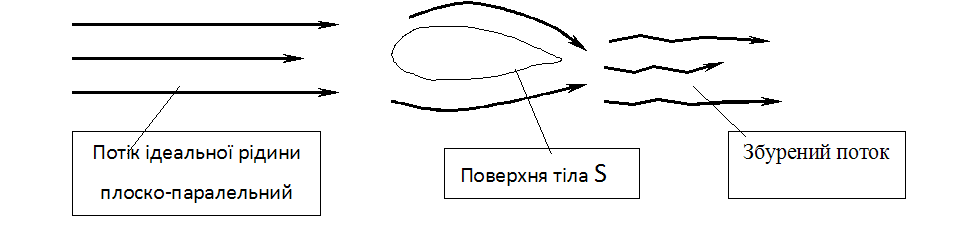
\includegraphics[width=\textwidth]{img/10-1.png}
\end{figure}

Через поверхню тіла потік не протікає це означає, що нормальна складова вектора швидкості дорівнює нормальній складовій вектору швидкості поверхні тіла $U_n$:
\begin{equation}
	\left. V_n(x, t) \right|_{x \in S} = U_n(x, t).
\end{equation}

Якщо тіло нерухоме, а потік набігає на тіло, то умова непротікання приймає вигляд
\begin{equation}
	\left. V_n(x, t) \right|_{x \in S} = 0.
\end{equation}

\subsubsection{Задача про поршень}

\begin{definition}[поршня]
	\it{Поршень} --- непрониклива для рідини поверхня, яка рухається в просторі, і при цьому може змінювати свою форму. 
\end{definition}

Задача про поршень узагальнює задачу обтікання тіла. Рівняння поверхні поршня запишемо у вигляді:
\begin{equation}
	h(x, t) = 0.
\end{equation}

На поверхні поршня повинна виконуватись умова непротікання. Запишемо її з використанням рівняння поверхні поршня:
\begin{equation}
	\diff h = \Sum_{i = 1}^3 \frac{\partial h}{\partial x_i} \cdot \diff x_i + \frac{\partial h}{\partial r} \cdot \diff t = 0.
\end{equation}

Позначимо $U_i = \diff x_i / \diff t$ --- складові вектора швидкості поверхні в напрямку вісі $Ox_i$. Вектор нормалі до поверхні поршня можна записати у вигляді
\begin{equation}
	\vec n = \frac{\nabla h}{\|\nabla h\|} = \frac{1}{\|\nabla h\|} \big( h_x, h_y, h_z \big).
\end{equation}

Тоді легко отримати нормальну складову вектору швидкості поверхні:
\begin{equation}
	\left( \Sum_{i = 1}^3 h_{x_i} U_i \right) \cdot \frac{1}{\|\nabla h\|} = U_n = - \frac{h_t'}{\|\nabla h\|}.
\end{equation}

Нормальна складова вектора швидкості рідини дорівнює:
\begin{equation}
	V_n = \left\langle \vec V, \vec n\right\rangle = \Sum_{i = 1}^3 \frac{V_i h_{x_i}}{\|\nabla h\|}.
\end{equation}

Прирівнюючи нормальну складову вектору швидкості поверхні і вектору швидкості рідини отримаємо граничну умову на поршні 
\begin{equation}
	- \frac{h_t'}{\|\nabla h\|} = \Sum_{i = 1}^3 \frac{V_i h_{x_i}}{\|\nabla h\|}.
\end{equation}

Або після скорочення
\begin{equation}
	\left. \frac{\partial h}{\partial t} + \Sum_{i = 1}^3 \frac{\partial h}{\partial x_i} \cdot V_i \right|_{x \in S} = 0
\end{equation}
--- гранична умова на поверхні $S$ поршня.

\subsubsection{Задача про вільну поверхню}

\begin{definition}[вільної поверхні]
	\it{Вільна поверхня} --- поверхня, яка розділяє дві ідеальні рідини, і форма цієї поверхні знаходиться в процесі розв'язку задачі, нехай $h(x, t)$ --- невідома функція, яка описує форму поверхні.
\end{definition}

Оскільки через вільну поверхню рідина не протікає то на цій поверхні виконується умова як і на поверхні поршня з невідомою функцією $h(x, t)$:
\begin{equation}
	\left. \frac{\partial h}{\partial t} + \Sum_{i = 1}^3 \frac{\partial h}{\partial x_i} \cdot V_i \right|_{x \in S} = 0
\end{equation}

Це додаткове рівняння для знаходження функції $h$. \medskip

Для знаходження додаткової невідомої функції $h$ на поверхні розділу середовищ задається розподіл тиску:
\begin{equation}
	\left. p(x, t) \right|_{x \in S} = P_a(x, t).
\end{equation}

Для випадку поршня і для випадку вільної поверхні початковий стан поверхні задається у вигляді:
\begin{equation}
	h(x, 0) = h_0(x).
\end{equation}

\subsubsection{Задача руху рідини в каналах}

\begin{definition}[каналу]
	\it{Канал} --- просторова область, яку можна утворити якщо переміщувати вздовж деякого незамкненого контуру в просторі нанизаний на нього замкнений контур змінної форми. В результаті утвориться область обмежена непроникливою для рідини поверхнею $S_3$, і проникливими для рідини поверхнями $S_1$, $S_2$ через які рідина може втікати або витікати:

	\begin{figure}[H]
		\centering
		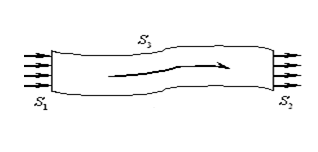
\includegraphics[width=.5\textwidth]{img/10-2.png}
	\end{figure}
\end{definition}

Як правило канали використовують для перетворення потоків. \medskip

Постановка граничних умов для течій в каналах має специфіку, яка визначається властивостями рівнянь руху ідеальної рідини (газової динаміки). Граничні умови на непроникливій поверхні $S_3$ є класичні умови непротікання. Вигляд граничних умов на поверхнях $S_1$ та $S_2$ залежить від швидкістю рідина на цих границях, а також від того втікає або витікає рідина з каналу. \medskip

Рухи рідини можна розділити на два режими:
\begin{itemize}
	\item $V_n > c$ --- надзвуковий режим руху (швидкий рух);
	\item $V_n < c$ --- дозвуковий режим руху (повільний рух).
\end{itemize}

\begin{remark}
	Тут $c$ --- термодинамічна скалярна величина, яка характеризує швидкість розповсюдження малих збурень (акустичних коливань) в рідині. Для визначення швидкості звуку використовується співвідношення
	\begin{equation}
		c^2 = \left. \frac{\partial p}{\partial \rho} \right|_{S = \const} > 0.
	\end{equation}
\end{remark}

При цьому рівняння стану зручно вибирати у вигляді $S = S(p, \rho)$.

\begin{enumerate}
	\item Розглянемо дозвукове втікання на поверхні $S_1$: $V_n < c$. \medskip   

	В цьому випадку необхідно задавати одну динамічну умову, наприклад потік маси через поверхню:
	\begin{equation}
		(\rho V_n )(x, t) = K \left. (p(x, t) - p_a) \right|_{x \in S_1}
	\end{equation}

	\begin{remark}
		Тут $p(x, t)$ --- тиск на поверхні $S_1$, $p_a$ --- атмосферний тиск, $(\rho V_n)(x, t)$ --- потік маси.
	\end{remark}

	\begin{remark}
		Оскільки рідина втікає, то $p_a > p(x, t)$.
	\end{remark}

	Друга гранична умова при дозвуковому втіканні потребує завдання однієї термодинамічної функції, наприклад ентропії:
	\begin{equation}
		\left. S(x, t) \right|_{x \in S_1} = S_i,
	\end{equation}
	або питомої внутрішньої енергії
	\begin{equation}
		\left. \epsilon(x, t) \right|_{x \in S_1} = \epsilon_i,
	\end{equation}

	\item Розглянемо дозвукове витікання на поверхні $S_2$: $V_n < c$. \medskip

	В цьому випадку достатньо задати лише одну граничну умову:
	\begin{equation}
		(\rho V_n )(x, t) = K \left. (p(x, t) - p_a) \right|_{x \in S_2}
	\end{equation}

	\begin{remark}
		Оскільки рідина витікає, то $p_a < p(x, t)$.
	\end{remark}

	\item Розглянемо надзвукове втікання на поверхні $S_1$: $V_n > 1$, \medskip

	При надзвуковому втіканні рідини на границі $S_1$ необхідно задавати усі п'ять функцій:
	\begin{equation}
		\left. \vec V \right|_{x \in S_1} = \vec V_i, \quad \left. \rho \right|_{x \in S_1} = \rho_i, \quad \left. p \right|_{x \in S_1} = p_i.
	\end{equation}

	\item Розглянемо надзвукове витікання через поверхню $S_2$: $V_n > c$. \medskip

	В цьому випадку ніяких граничних умов на відповідній границі ставити не треба, рідина, яка \bf{дуже швидко} витікає через $S_2$ ніяк не впливає на внутрішню течію в каналі.
\end{enumerate}

\end{document}